\section{Critique of Evaluation Practices}
\label{sec:methodology}

The three failure patterns of Section~\ref{sec:failure} are partly enabled
by a weak evaluation culture in the GrC feature-selection literature.
We document four recurring problems and propose minimum reporting standards.

%-----------------------------------------------------------------------
\subsection{The 3-NN/SVM-UCI Benchmark Is Insensitive}
\label{sec:insensitive}
%-----------------------------------------------------------------------

The dominant evaluation protocol in the field is: run forward-greedy
attribute reduction with a proposed significance measure; select the top-$k$
attributes; evaluate 3-NN or SVM-RBF on UCI datasets; report mean accuracy.
This protocol has a structural defect: on many UCI datasets, the baseline
of selecting \emph{all} features is competitive with or superior to the best
reduct---and that baseline is usually not reported, so the reader cannot see
the problem.  In the full-text coding of Table~\ref{tab:practice}, 17 of the
22 papers omit it---10 of the 13 that belong to our Axis-1 corpus.

Table~\ref{tab:allfeats} shows the best-$k$ accuracy achieved by any method
versus the all-features baseline on our ten-dataset benchmark.

% AUTO-GENERATED by gen_tables.py -- do not edit by hand.
% Regenerate:  python3 gen_tables.py   Audit:  python3 verify_tables.py
\begin{table}[pos=!htbp]
\caption{Best-$k$ 3-NN accuracy (maximised over methods and
$k \in \{1,\ldots,d\}$) versus all-features baseline.  Mean $\pm$ SD over
5~folds $\times$ 5~seeds.  $\Delta$ is the margin in percentage points;
$p_{\mathrm{Holm}}$ is a paired Wilcoxon signed-rank test over the 25
matched fold--seed pairs, Holm-corrected for the ten comparisons.
$\dagger$ marks the dataset where best-$k = d$, i.e.\ no strict subset
outperforms the full feature set.}
\label{tab:allfeats}
\centering\small
\setlength\tabcolsep{4pt}
\begin{tabular}{lrrccrrr}
\toprule
Dataset & $n$ & $d$ & All-feat acc. & Best-$k$ acc. & $k^*$ & $\Delta$ (pp) & $p_{\mathrm{Holm}}$ \\
\midrule
Iris       & 150 &  4 & $94.4 \pm 4.9$\% & $96.1 \pm 3.9$\% & 3 & $+1.73$ & $0.078$ \\
Wine       & 178 & 13 & $96.0 \pm 2.8$\% & $97.3 \pm 2.8$\% & 9 & $+1.35$ & $0.167$ \\
Ionosphere & 351 & 34 & $84.9 \pm 3.9$\% & $90.4 \pm 3.9$\% & 5 & $+5.48$ & $<0.001$ \\
Sonar      & 208 & 60 & $84.2 \pm 6.8$\% & $84.7 \pm 7.1$\% & 38 & $+0.47$ & $1.000$ \\
Glass      & 214 &  9 & $68.5 \pm 5.5$\% & $73.4 \pm 6.1$\% & 7 & $+4.85$ & $0.005$ \\
Ecoli      & 336 &  7 & $84.5 \pm 3.7$\% & $84.6 \pm 3.6$\% & 6 & $+0.06$ & $1.000$ \\
Heart      & 270 & 13 & $81.5 \pm 5.1$\% & $81.5 \pm 5.1$\% & 13$\dagger$ & $+0.00$ & $1.000$ \\
Parkinsons & 195 & 22 & $91.4 \pm 3.6$\% & $93.4 \pm 3.9$\% & 15 & $+2.05$ & $0.006$ \\
Seeds      & 210 &  7 & $92.5 \pm 3.6$\% & $93.1 \pm 3.3$\% & 4 & $+0.67$ & $1.000$ \\
WDBC       & 569 & 30 & $96.6 \pm 1.5$\% & $97.0 \pm 1.3$\% & 16 & $+0.46$ & $0.911$ \\
\bottomrule
\end{tabular}
\end{table}


The margins are small: seven of the ten datasets gain at most $2$ pp from
the best reduct over the whole feature set, and on Heart the best reduct
is the whole feature set.  Rather than declare a noise threshold by
inspection, we test each margin.  A paired Wilcoxon signed-rank test over the
25 matched fold--seed pairs, Holm-corrected for the ten comparisons, finds
the gain significant on only three datasets: Ionosphere ($+5.5$ pp),
Glass ($+4.9$ pp) and Parkinsons ($+2.1$ pp).  On the remaining seven the
best reduct that any of the seven methods can produce is statistically
indistinguishable from using every feature.
Figure~\ref{fig:margin} visualises the margins with this distinction.

The consequence for the field is the important part.  If the best
selector at the best $k$ cannot separate itself from the do-nothing
baseline on seven of ten standard benchmarks, then a comparison between two
selectors on those benchmarks is being conducted inside the interval where
the benchmark has no resolving power.  This is a property of the evaluation
protocol, not of any particular method, and it applies equally to our own
PAI results in Section~\ref{sec:failure}: the PAI-versus-NRS gaps we report
are large enough to survive it, but many published gaps are not.

\begin{figure}[pos=!htbp]
\centering
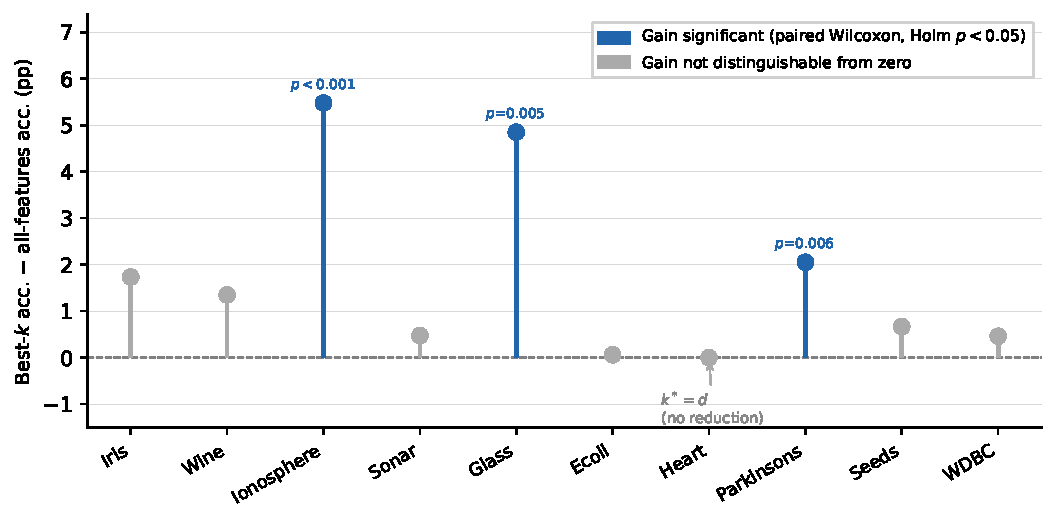
\includegraphics[width=\columnwidth]{figures/margin_plot.pdf}
\caption{Best-$k$ 3-NN accuracy minus the all-features baseline per
dataset (lollipop chart).  Blue: the gain is significant under a paired
Wilcoxon signed-rank test over the 25 matched fold--seed pairs after Holm
correction for the ten comparisons ($p<0.05$, value annotated); grey: the
gain is not distinguishable from zero.  Seven of ten datasets are grey,
so between-method comparisons at this benchmark scale are largely
uninformative.}
\label{fig:margin}
\end{figure}

%-----------------------------------------------------------------------
\subsection{Significance Testing Is Rare}
\label{sec:significance}
%-----------------------------------------------------------------------

Statistical testing is rare in the GrC feature-selection literature.
Zhang et al.~\cite{Zhang2023GiniNRS} state in their own paper---which proposes
a Gini-enhanced NRS variant and reports improvements on 16 UCI
datasets---that ``\emph{statistical tests reveal no significant differences
between the proposed algorithm and the four classical neighborhood rough
set-based feature selection algorithms}.''  The paper is published as an
improvement regardless.  This is not an isolated case: it reflects the
community's structural tolerance for non-significant comparisons on
low-sensitivity benchmarks.

\paragraph{How common is this?  A full-text coding.}
Answering this requires reading experimental sections, not abstracts.  We
read 22 attribute-reduction papers at full text and coded four
presence/absence facts from each paper's experimental section.  Thirteen of
them are members of this survey's Axis-1 corpus, and they are 13 of the 25
Axis-1 papers---so for the axis that dominates recent output
(Figure~\ref{fig:activity}) this is a majority coding, not an anecdote.
Table~\ref{tab:practice} reports the counts for both groupings, and
Table~\ref{tab:practice_detail} gives the per-paper judgements for the
corpus members.

% AUTO-GENERATED by gen_tables.py -- do not edit by hand.
% Regenerate:  python3 gen_tables.py   Audit:  python3 verify_tables.py
\begin{table}[pos=!htbp]
\caption{Reporting practice in attribute-reduction papers read at full text.
Each cell is a presence/absence judgement made from the experimental section
only; the coding and the supporting quotation for every cell are released as
\texttt{fulltext\_coding.csv}.  Column~2 covers all 22 papers
coded; column~3 restricts to the 13 that are members of this
survey's Axis-1 corpus (Appendix~\ref{app:search}), i.e.\ 13
of the 25 Axis-1 papers.}
\label{tab:practice}
\centering\small
\begin{tabular}{lcc}
\toprule
Practice & All coded ($n=22$) & Axis-1 corpus ($n=13$) \\
\midrule
All-features baseline reported & 5/22 & 3/13 \\
Dispersion (SD or per-fold) reported & 6/22 & 2/13 \\
Statistical significance test run & 12/22 & 7/13 \\
Own hyperparameter ablated & 7/22 & 3/13 \\
\midrule
\textbf{All four} & 0/22 & 0/13 \\
\textbf{None of the four} & 5/22 & 3/13 \\
\bottomrule
\end{tabular}
\end{table}


Within the Axis-1 corpus, 10 of 13 papers report no all-features baseline, so
a reader cannot tell whether selection helped at all; 11 of 13 report no
dispersion, so no reader can run the paired test the paper omitted; and 10 of
13 vary no hyperparameter of their own method.  Seven of 13 run a
significance test.  Three papers report none of the four practices.  Across all 22 papers
coded, \emph{not one reports all four}.

The single most consequential gap is the missing baseline.  Section~\ref{sec:insensitive}
showed that on seven of ten benchmarks the best reduct any method can produce
is statistically indistinguishable from keeping every feature.  A paper that
does not report the all-features number cannot detect that it is in this
regime, and neither can its reviewer.

\paragraph{What this coding can and cannot support.}
We state the limits precisely, because the alternative is the error this
section criticises.  The papers are those we could obtain in full text, not a
random draw, and they concentrate in the granular-ball and fuzzy-neighbourhood
branch: the Axis-1 figures generalise to Axis~1, not to Axes~2--4, which we do
not claim to have coded.  Counts are reported as fractions rather than
percentages of the field.  The coding records only whether a practice is
present, not whether it was done well---a paper credited with a significance
test may still have applied an inappropriate one, and one paper's test is run
on runtime rather than accuracy.  Judgements are deliberately conservative:
a mention of the ``original dataset'' in a method description or a figure
caption is not counted as a baseline, and tuning a comparison classifier's
$k$ is not counted as ablating one's own hyperparameter.  Every cell carries
the quotation it rests on, so an individual judgement can be overturned
without re-reading the paper.

A broader pattern is visible from our own evaluation: a 3-NN accuracy
difference of 1\% on a dataset of $n \leq 300$ objects corresponds to a
shift of 2--3 objects between folds, which is within the variance of a
single run.  Reporting means without standard deviations, and means without
a paired test across datasets, provides no evidence that a measured difference
exceeds noise.  Feature selection reviews in the ML literature~\cite{Saeys2007}
document the same insensitivity: no single filter or wrapper method dominates
across UCI benchmarks, and small-sample variance is the primary confound.

\paragraph{Minimum standard.}
Any claim of superiority over a baseline requires:
(a) per-fold accuracy (not just means), so a paired test is possible;
(b) a paired Wilcoxon signed-rank test across datasets or folds;
(c) effect size ($|\Delta \text{acc}|$, not just $p < 0.05$).

%-----------------------------------------------------------------------
\subsection{No Ablation of Generator Parameters}
\label{sec:ablation}
%-----------------------------------------------------------------------

GBNRS-family methods have one key hyperparameter: purity threshold $\tau$
(default $2/3$).  NRS methods have radius $\delta$.  Persistence-based
methods have filtration maximum $\varepsilon_{\max}$ and maximum homological
dimension $d_{\max}$.  Ablation of these is rare: in the full-text coding of
Table~\ref{tab:practice}, 15 of 22 papers vary no hyperparameter of their own
method, several stating a fixed value in passing---``the purity is set to
1''---without reporting what happens at any other setting.  The exceptions
show it is neither hard nor expensive: one sweeps the purity threshold from
$0.54$ to $1.0$ in fixed steps, another reports results for
$K \in \{1,\ldots,7\}$, and a third devotes a subsection to parameter
sensitivity.

Without ablation, it is impossible to determine whether an observed
improvement is due to the proposed mechanism or to an implicit
hyperparameter choice that happens to suit the benchmark datasets.
The filter-versus-wrapper distinction~\cite{KohaviJohn1997} is relevant here:
NRS-based significance measures are pure filter criteria, and showing that the
proposed measure is robust to the hyperparameter (rather than merely tuned for it)
is the filter-method equivalent of wrapper stability.

The point extends to a place the field almost never looks: the free
parameters of the \emph{evaluation metric}, not just of the method.
Section~\ref{sec:patC} gives a worked instance.  The structure-preservation
metric \texttt{knn\_overlap} takes a neighbourhood size $K$, conventionally
left at a default of $10$ and never varied.  Ablating it
(Table~\ref{tab:knn_scale}) moves PAI's advantage over NRS from significant
($p=0.037$ at $K=5$) through borderline ($p=0.064$ at $K=10$) to reversed
($K=50$), on identical feature subsets.  A paper reporting only the default
would state a significant structural advantage or none at all depending on a
choice its authors likely never registered as a choice.  Metric
hyperparameters deserve the same ablation as method hyperparameters.

We acknowledge the same gap in our own experiments: PAI uses a single
filtration setup (Vietoris--Rips, $d_{\max}=1$, max threshold $=2.0$) and
NRS uses a fixed $k=7$ throughout, without varying these parameters.
A full ablation of $k$ and $d_{\max}$ is beyond the scope of this survey's
experimental programme but is noted as a limitation
(Section~\ref{sec:limitations}).

%-----------------------------------------------------------------------
\subsection{Negative Results Are Suppressed}
\label{sec:negative}
%-----------------------------------------------------------------------

Our own experimental programme generated several negative results:
\begin{itemize}
  \item Persistence-based attribute importance does not complement
        NRS on 10 UCI datasets (Fisher-$z$ $\bar\rho = -0.060$, 95\% CI
        $[-0.21,\,+0.09]$; Section~\ref{sec:patB}).
  \item PAI is statistically indistinguishable from a variance-based null
        baseline on 3-NN ($p = 0.23$; Section~\ref{sec:patB}).
  \item A PAI/NRS hybrid ranking does not rescue PAI ($p = 0.010$ vs NRS;
        Section~\ref{sec:patB}).
  \item Persistence-based selection loses to NRS on trustworthiness
        ($p=0.006$) and cluster ARI ($p=0.004$), dataset-level Wilcoxon
        $n=10$ (Section~\ref{sec:patC}).
  \item All findings replicate under SVM-RBF evaluation ($p = 0.006$;
        Section~\ref{sec:patB}).
  \item The one metric on which PAI appeared to lead---\texttt{knn\_overlap}
        ---reverses sign when the metric's own neighbourhood parameter is
        varied from $K=5$ to $K=50$ on unchanged feature subsets, and the
        scale-matching mechanism we had proposed to explain the lead is not
        supported by the data ($\rho = -0.10$, $p = 0.80$;
        Section~\ref{sec:patC}).
\end{itemize}

These findings are not reported elsewhere in the literature because
experiments that confirm a null result are rarely submitted.  The net
effect is a bibliography that reads as uniformly positive, which
misleads researchers choosing between directions.

We release all raw results per fold per seed so that future surveys can
use them as a negative-result baseline.

%-----------------------------------------------------------------------
\subsection{Minimum Reporting Standard}
\label{sec:standard}
%-----------------------------------------------------------------------

We propose the following minimum standard for GrC feature-selection
experimental papers, modelled on reporting norms in NLP and CV:

\begin{enumerate}
  \item \textbf{Include an all-features baseline.}  Report accuracy with
        no selection as a reference baseline; this reveals whether
        dimensionality reduction helps at all on the benchmark.
  \item \textbf{Report per-fold accuracy.}  This enables paired
        significance tests by downstream readers even if the paper
        does not run them.
  \item \textbf{Apply a paired Wilcoxon or Friedman/Nemenyi test}
        \cite{Demsar2006,Garcia2010IS}.
        Report effect size alongside $p$-value.
  \item \textbf{Ablate at least one generator hyperparameter---and every
        free parameter of the evaluation metric.}  Show that the result is
        not an artefact of a default setting.  Metric parameters
        (neighbourhood sizes, cluster counts, kernel widths) are the
        commonest unexamined defaults and can reverse a conclusion on
        unchanged data (Table~\ref{tab:knn_scale}).
  \item \textbf{Separate timing.}  Report reduct-finding time and
        evaluation time separately; the former is the method's cost,
        the latter is fixed.
  \item \textbf{Register negative outcomes.}  If a method is tried and
        fails (against the paper's hypothesis), note it in the paper
        rather than omitting the experiment.
\end{enumerate}

These standards add approximately half a page to a paper but substantially
increase the information content and reliability of the result.
